Theory here, in present tense.

This is an equation
\begin{align} \label{theo:eq:newton2}
    F = ma.
\end{align}

We cite our sources like this~\citep{Project1}.

\subsection{Principal Component Analysis (PCA)}

    \subsubsection{Motivation and assumptions}
        Consider the collection of data $X$ which is a $(n\cross m)$ matrix, with $n$ data points, and $m$ features. We might find ourselves in a situation where some features are highly correlated. As a result, some features might be considered obsolete since the trend they describe can easily be described by other features, or combinations of other features. If this is the case, then $X$ contains more features than is strictly necessary in order to explain the trends in the data. Principal component analysis is a technique where we make linear combinations of the original features in such a way that we can describe the data with as few as possible of these new features, effectively reducing the dimensionality of the problem, without loosing too much information about the data itself. By doing this we can perform the computations with a dataset of fewer dimensions, increasing the computational efficiency. We assume that we can describe the data by its variance only. This implies that the mean must be zero, i.e. the data must be in mean-deviation form. We also assume the data to be normally distributed, as a mean-centred normal distribution is the only distribution described by its variance alone.
        
        \begin{figure}
            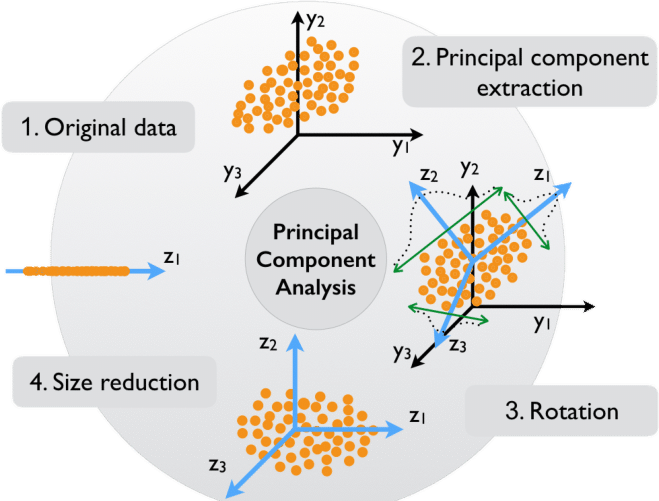
\includegraphics[width=\linewidth]{figs/pca_schematic.png}
            \caption{Schematic representation of PCA. New axes, represented as $z$ in the figure are generated, forming a new basis and a new hyperplane onto which we project the data in order to maximise variance and minimise covariance.\citep{pca_img}}
            \label{theo:fig:pca_schematic}
        \end{figure}
        
        From a geometrical point of view, this can be thought of as expressing the data in a different coordinate system, and PCA involves determining these new axes. Figure \ref{theo:fig:pca_schematic}  shows a visual interpretation of this, where the black axes are the original ones, and we find the new blue axes with PCA. These are determined in such a way that the variance of the data is maximised in the new coordinate system, while minimising the covariance between features. We must impose this criterion since we want as few new features as possible, hence we do not want them to co-vary, but rather vary as much as possible. 

    \subsubsection{Mathematical consideration}

    Our goal is to reduce the dimensionality of the data, thus we want to represent the data as a matrix $Y$ with shape $(n\cross d)$ where $d\leq m$. This indicates that we are after a linear transformation $T:\mathbb{R}^{n\cross m} \to \mathbb{R}^{n\cross d}$ which we can define by $T(X) = XP = Y$, where $P$ is an orthonormal matrix of shape $m\cross d$, which we intend to find. $P$ must fulfil our criterion on $Y$, which is high variance and low covariance. This can be done by diagonalising the covariance matrix of $Y$ given by:

    \begin{align}\label{theo:eq:Y_covariance}
        S_Y &= n_cY^TY\nonumber\\
        &= n_c(XP)^T(XP) \nonumber\\
        &= n_cP^T(X^TX)P,
    \end{align} 
    where $n_c = 1/(n-1)$ is the normalisation due to $n$ data points.

    With \citep[ch. 5.3]{linalgbok} we can show that any square symmetric matrix, like $X^TX$, can be expressed as $EDE^T$ where the columns of $E$ are the orthonormal eigenvectors of $X^TX$, and $D$ is a diagonal matrix. Inserting this into equation  \ref{theo:eq:Y_covariance} we obtain that $S_Y = n_cP^TEDE^TP$. We see that $P=E \implies S_Y=n_c D,$\footnote{This is not necessarily trivial since we want $P$ to have shape $(m\cross d)$. $E$ contains all the eigenvectors of $X^TX$ and has thus shape $(m\cross m)$. This is easily surpassed by setting $d=m$ while showing this, and then reduce the dimension of $P$ when we need it later. We also note that this works mathematically if we let $E$ contain the $d$ eigenvectors of $X^TX$ with the largest eigenvalues. Then $D$ must be a $(d\cross d)$ diagonal matrix, which is of similar shape as $S_Y$.} since $P$ is then orthonormal and thus $P^T=P^{-1}$.
 
    % \footnotetext{This is not necessarily trivial since we want $P$ to have shape $(m\cross d)$. $E$ contains all the eigenvectors of $X^TX$ and has thus shape $(m\cross m)$. This is easily surpassed by setting $d=m$ while showing this, and then reduce the dimension of $P$ when we need it later. We also note that this works mathematically if we let $E$ contain the $d$ eigenvectors of $X^TX$ with the largest eigenvalues. Then $D$ must be a $(d\cross d)$ diagonal matrix, which is of similar shape as $S_Y$.}

    Hence, choosing the columns of $P$ to be the orthonormal eigenvectors of $X^TX$ yield a diagonal covariance matrix $S_Y$, exactly what we want. This link can also be made through the singular value decomposition (SVD). We can express any matrix $X$ as $X=U\Sigma V^T$ \citep[ch. 7.4]{linalgbok}, where $V$ is a matrix containing the orthonormal eigenvector of $X^TX$. Without delving further into SVD, we see that $P$ may also be found from the column vectors in $V$. 
    
    We conclude that the principal components of $X$ can be expressed as $P=[\vec{p}_1, \dots \vec{p}_d]$, where $\vec{p}_1$ is the eigenvector of $X^TX$ that corresponds to the largest eigenvalue, $\vec{p}_2$ to the second largest and so on. This continues until we have found $d$ principal components. Each $\vec{p}_i$ is by construction a linear combination of the original features and has shape $(m\cross 1)$.   The elements of PCA may then be summarised as follows:

    \begin{enumerate}
        \item Make sure $X$ has shape $(n\cross m)$ and is in mean-deviation form.
        \item Find $P$ either from $V$ or the eigenvectors of $X^TX$ directly.
        \item Calculate $Y=XP$.
        \item Find the diagonal covariance $S_Y=n_cY^TY$.
    \end{enumerate}
    
    \subsubsection{Interpretation}
    Now we have a recipe of finding the principal component $P$, but what do they really mean? We perform PCA in order to reduce the redundancy of features, to express the data with as few features/dimensions as possible without loosing too much information. We therefore make new features that are linear combinations of the original features, but with zero covariance. This means that when we ``choose'' the first principal component $\vec{p}_1$, we find the direction in feature space, along which the variance of the data is maximised. In other words, if we were to project all data points down on a line, $\vec{p}_1$ would be the line that gives the largest variance, i.e. yield as much information about the data as possible for a 1D data set. When finding the next principal component we repeat this process, but restrict ourselves to only ``choosing'' directions in feature space orthogonal to the previous. 
    
    Having $d$ principal components means that we have found $d$ directions in feature space, all with a maximised variance. These can be though of as a new basis or representing our data $X$. Then the matrix $P$ can be interpreted as the change of basis matrix between $X$ and $Y$. $Y$ are the same data points, but expressed in the basis of the principal components. They are the data points projected onto a hyperplane set up by the vectors $\vec{p}_i$. This can also be inferred from figure \ref{theo:fig:pca_schematic}. We also notice a rather neat consequence of the SVD, that finding the principal components of $X$ equates to finding an orthonormal basis that span $\text{Row}(X)$. The $i$-th diagonal element of $S_Y$ is the variance, $\sigma_i^2$ of the data along $\vec{p}_i$. The total variance is the sum over these diagonal elements, or the trace, $\text{tr}(S_Y)$.

     

\subsection{Neural Networks}
    First, it will be wise to take a minute to recap some of the details of how a \textit{feed-forward nerual network} (FFNN) is built and trained from~\cite{Project2}. They are made up of sequential \textit{layers} taking in the input from the previous layer and passing it on to the next one. There will always be an input layer, taking in the features $x$ producing some observation $y$, and an output layer transforming the input from the second to last layer into an appropriate output. In classification problems, the outputs will usually be probabilities $p_c$ between $0$ and $1$ for the input to produce an output in a given category $c$. In regression, the output layer usually transforms the output to be a single number $\tilde{y}$ for the predicted value.

    When passing the output from one layer as input to the next, a linear transformation is done. Denoting the output vector from layer $\ell$ as $\vec{a}^\ell$, the transformation produces a \textit{response} $\vec{z}^{\ell} = W^\ell \vec{a}^{\ell-1} + \vec{b}^\ell$, where $W^\ell$ is a weight matrix with elements $w^\ell_{ij}$, and $\vec{b}^\ell$ is called the bias.\footnote{Here $i$ enumerate the component nodes of the current layer, and $j$ enumerate the inputs to the layer.} The response vector is then passed through an activation function (which is generally non-linear) to produce the \textit{activation} $\vec{a}^\ell = f(\vec{z}^\ell)$.

    Now introducing some new terms, when referring to a node with activation $a^\ell$, the corresponding weights $W^\ell$ will be referred to as the \textit{incoming weights}, and $W^{\ell + 1}$ as \textit{outgoing weights}.

\subsection{Neurological Background: Competing Neurons}
    The first artificial neural networks were inspired by biological neurons (cells mainly located in the brain); artificial nodes represent the neurons and their activation, the weights represent the synapses (connections between neurons), and biases address the threshold for activation of each neuron/node~\citep{Project2}. Since then, the development of neurobiologically inspired artificial intelligence has only increased and many other algorithms mimicking mechanisms of the brain have been employed to enhance machine learning performance. An up-and-coming and interesting field of research is the implementation of biological competative mechanisms. 
    
    First some important terms. Biological neurons are often considered to be either activated or not activated; a binary state of either on or off. Neurons are activated by receiving sufficient signals from sensory receptors or other activated neurons. When an activated neuron passes on its signal to another neuron, that signal can be either \textit{excitatory}, nudging the second neuron towards activation, or \textit{inhibitory}, reducing the chances of activation. \comment{should perhaps have a source} A series of activated neurons can be considered a pathway created in the brain, and there exists a consensus that information in the brain is represented, not by the signal within a cell (which is very similar for all cells and therefore convey little information), but rather through the signal's pathway between cells \comment{(Kandel)}. It is hypothesised that some of these pathways arise through competition between adjacent neurons. \comment{source plis, perhaps Self-organized formation of topologically correct feature maps}
    
    \subsubsection{Lateral Inhibition}

        An example of competative mechanisms that are present in neurobiological systems is a phenomenon referred to as \textit{lateral inhibition}. It exhibits the competative selectivity between neurons and neural pathways. This is assumed to enhance the sense of contrast and is present especially in sensory procedures. The mechanism behind lateral inhibition is that the neurons receiving the most sensory input inhibit the activity of the neurons in close proximity (radius from 200 to 500 \textmu m), making themselves the "winners" and the nearby neurons the "losers". For example, when neurons receive input from receptors of some external stimuli, the neurons connected to the most stimulated receptors will inhibit the nearby neurons connected to less stimulated receptors, making them less likely to be activated. This will lead to the outer part of the stimulus being toned down and the central stimulus appearing stronger in contrast. \textit{This is a basis for the winner-takes-all models which will be further dicussed later.}
        \comment{Need some source on the mechanism} 
        
        There exists both anatomical an physiological evidence supporting the theory of lateral inhibition (\comment{self-organised...}). It is hypothesized that between the competing neurons the inhibition occurs through inhibitory interneurons connecting the two neurons together.
        

    \subsubsection{Function}
        \comment{Present the unanswered questions. Why is this important in the brain? Implicit: what can we expect from our nns (Next section)}
       \textit{As the previous section states, the competative mechanism lateral inhibition correlates with the perception of contrasts. However}, there are also other neurological and even higher-level cognitive functions which might be explained or at least modelled by competition within the brain.

        As mentioned, in the brain information is conveyed through different patterns of neural activation in the form of neural pathways. Assuming this, an interesting question is how these neuronal pathways arise. One hypotesis is that the competition between neurons initially leads to various pathways which then are enforced by placticity in synapses. 
        
        The brain receives vastly different input at all times, and the mechanisms behind its ability to make distictions between these inputs are unknown. However, the \comment{almighty, hehe} hypothesis is that the answer lies in the neural activity. Supporting this hypothesis is the fact that variance in neural activty correlates with variance in input, suggesting some information is encoded here. In that case, if all neurons were to fire identically to all type of stimuli, no information would be encoded in the activity.

        
        
        
        \subsubsection{Function 2.0}
        In addition to enhancing contrast there are other neurological functions, and even higher-level cognitive functions which can be modelled by implementing the concept competition within the brain \citep{Chen}.
        
        Competition between neurons is hypothesised to \comment{heavily impact} the creation of biological neural pathways (Kohonen).
        As previously mentioned, neural pathways are series of activated neurons. These pathways are important as they are considered a manner of conveying information in the brain; assuming information is in some way encoded in brain activity, it follows that simultaneous and/or constant activation of all neurons will convey no information, and that pathways are necessary \citep{Chen}. When neurons compete, it will prevent neurons from all firing simultaneously and rather create sparse pathways. 
        Furthermore, the pathways are hypothesised essential in the brain for making useful distinctions between input, and develop so-called feature selectivity \citep{Chen}. Assuming that a certain pathway encodes part of the input, called a feature, competition between pathways leads to only some features being processed. 
        
        The immense amount of input, both external and internal, the brain receives at any given moment cannot be processed; somehow the brain prioritises the input. One hypothesis is that the competition between neural pathway leads to only some of the information being processed; only the winning neural pathways are activated \citep{Chen}. This hypothesis coincides with an intutive understanding of the concept of prioritising. While it should be mentioned that some information processing is assumed to be decided by higher-level cognitive functions, like attention \comment{source}, competition based on \textit{current} stimuli and established neural structures seems plausible; only the input which is most pressing and coherent with previously important input is processed.    
        
        Higher-level cognitive functions. 

    \subsubsection{Connect to ML/What can be expected from machine learning algorithms/ artificial neural networks mimicking biological competative mechanisms}
        Visual perception. 
        What has been seen in ML before (compete to compute)

\subsection{Local Winner-Takes-All (LWTA)}
    The idea behind LWTA algorithms is to implement \textit{local learning} in the neural network, meaning that the entire network does not learn how to transform a given input, but the learning is rather outsourced to local parts of the network. In LWTA algorithms, the nodes in each layer are grouped into a number of groups $G$, and Winner-Takes-All is applied on the activation of each of these groups, only passing on the maximal output in the group. This creates various neural pathways which learn during training, and are selected at inference time. The hypothesis is that different pathways get specialised in recognising different features of the training data and that a pathway will be activated given a datapoint with similar features as it is trained on, making the network more flexible and better at separating input \citep{Wang}. 

    Two different LWTA algorithms will be employd in this report: maxout, where pathways are only formed posteriori; and channel-out, where they are also formed anteriori.

    \subsubsection{Maxout and Channel-Out}
        The \textit{maxout} activation passes the input from the previous layer through the weight kernel and adds the bias as normal, but then only passes on the activation from the most active node in each group of the layer. Each group then has a common set of output weights connected to the next layer in  the network.See \cref{the:fig:illustration_maxout} for illustration of a neural network with maxout actvation.
        During backpropagation in training, only the incoming weights connected to the most activated nodes will be trained. This can be seen from the gradient of the cost function in the direction of one of the weights of an inactive node: the learning is proportional to $\pd[w^{\ell}_{ij}]{C} \propto \pd[a^\ell_i]{C} = 0$, because any infinitesimal change in the activation would still result in no activation if $a_i$ was not already the maximum of the group. 
        Given a datapoint, the neural pathways created through this algorithm consist of weights and nodes (see \cref{the:fig:illustration_maxout} for an example of pathways). The relevant nodes of a pathway are chosen based on which activation is largest within a group, and the input weights corresponding to those nodes are consequently chosen \citep{Wang}. 
        
        \begin{figure}[]
            \centering
            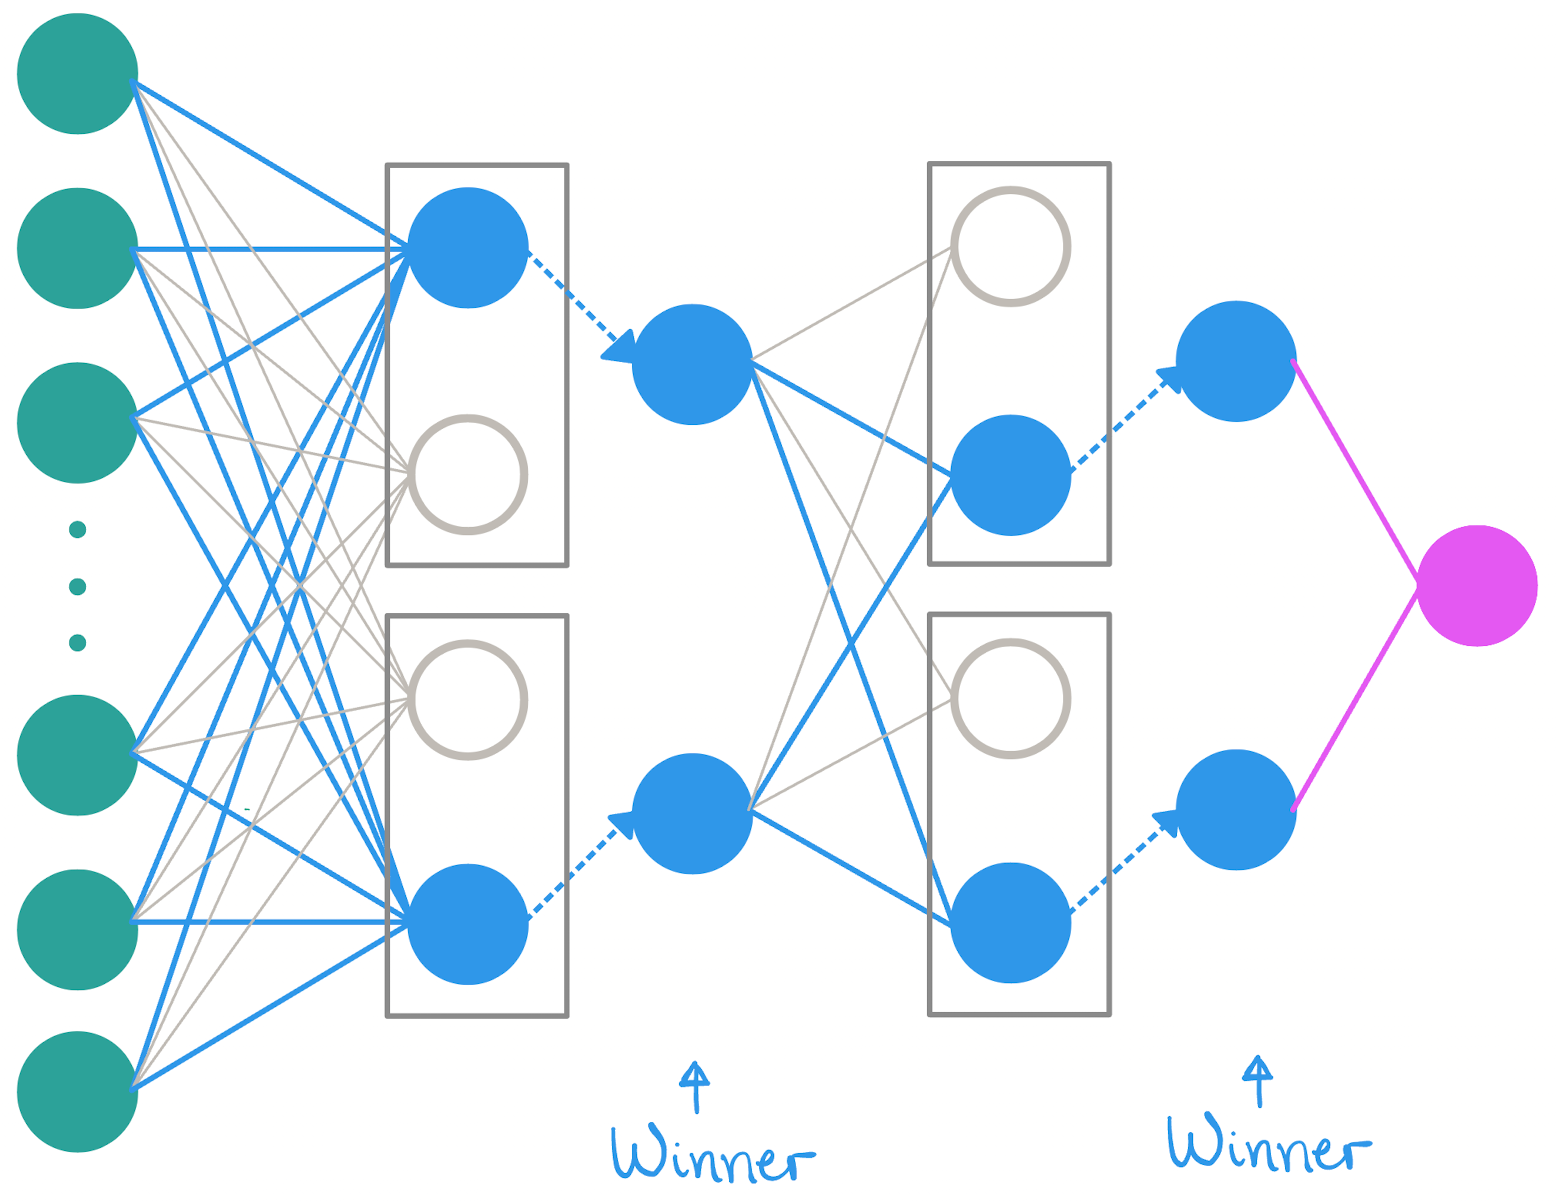
\includegraphics[width=\linewidth]{illustration_maxout.png}
            \caption{Illustration of a neural network with maxout. }
            \label[fig]{the:fig:illustration_maxout}
        \end{figure}


        % \begin{algorithm}
        %     \caption{Max Out activation}
        %     \begin{algorithmic}[1]
        %         \For{$i=1$ to $g$}
        %             \State $a_i \gets -\infty$
        %             \For{$j=1$ to $n \bmod g$}
        %                 \If{$z_{ij} > a_i$}
        %                     \State $a_i \gets z_{ij}$
        %                 \EndIf
        %             \EndFor
        %         \EndFor
        %     \end{algorithmic}
        % \end{algorithm}

        \textit{Channel-out} makes a subtle, but meaningful, change to the maxout algorithm. Instead of every group having a common set of weight connections to the next layer, every node has its own set of weight connections. This results in not only local learning of the weights during backpropagation, but also leads to the activation winner dictating the set of weights that will be used in the next layer at inference time (outgoing weights).
        Effectively, a channel-out layer works the same way as an ordinary dense layer with a linear activation function, but sets all the activations of the nodes that do not win their group to zero before passing them on to the next layer.
        Same as with maxout, only the weights of the active nodes are trained, but this also applies to the next layer; it not only affects the incoming weights, but also the outgoing weights.  
        So the local learning goes both forwards and backwards from a channel-out layer, in contrast to just backwards in the case of maxout \citep{Wang}. 
        \comment{In this case there exist more weights that are not trained as all nodes have their own outgoing weights.. Comment on the different number of parameters even though the same number of weights are trained in each iteration (given the same number of layers, nodes and groups)}
        
        \begin{figure}[]
            \centering
            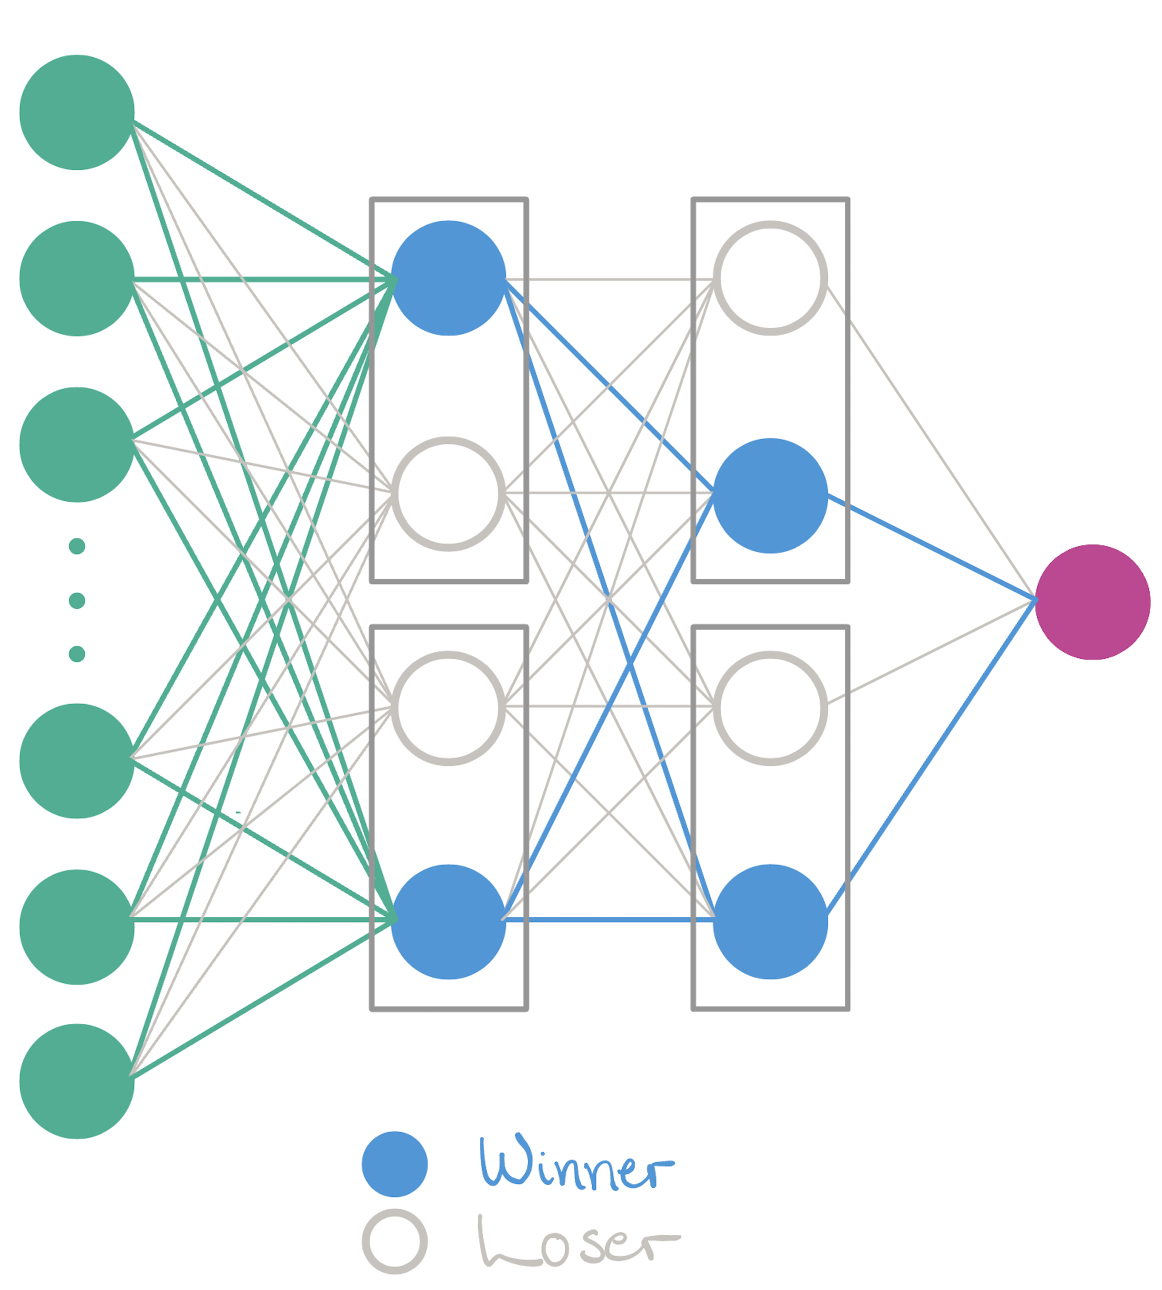
\includegraphics[width=.8\linewidth]{illustration_channelout.png}
            \caption{Illustration of a neural network with channel-out.}
            \label[fig]{the:fig:illustration_channelout}
        \end{figure}

        A way to look at the function of the LWTA groups is to study the effective activation output of the group. Simplifying by looking at a group of nodes whose input is only one scalar quantity $x$. The response of the nodes in the groups are linear functions $z_i = w_i x + b_i$ of the input, and the activation output is $\operatorname{max}(z_i)$. \cref{the:fig:activation_imitation} illustrates how the maximum of a group of such functions can mimic and parameterise different convex function. In fact, it is shown that a group of an arbitrary amount of nodes can approximate any convex function \citep{Maxout_Networks}.

        \begin{figure}[]
            \centering
            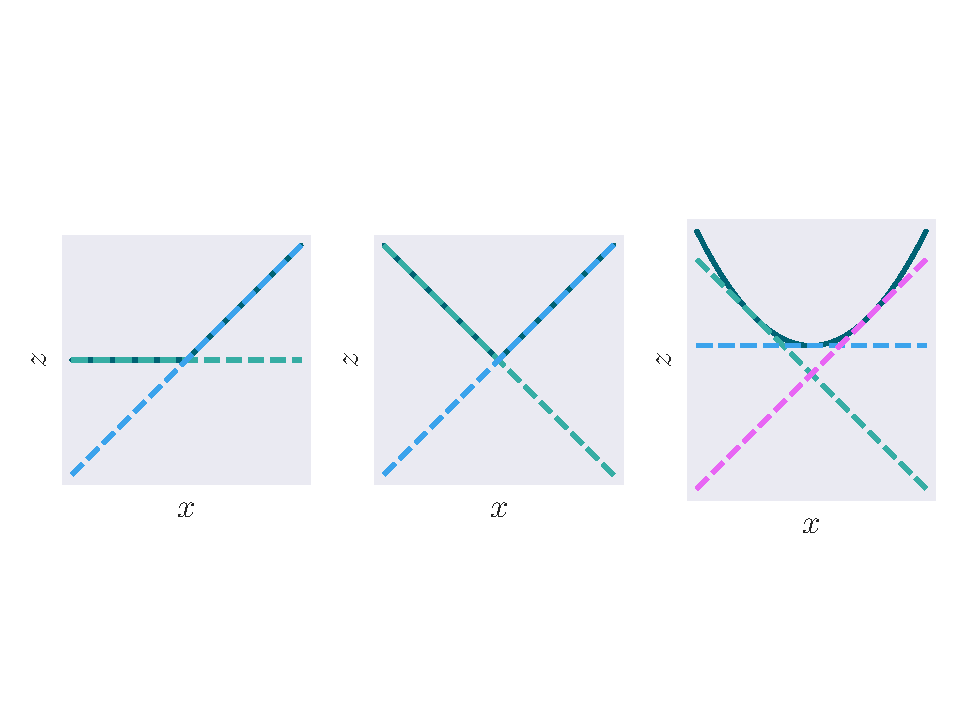
\includegraphics[width=\linewidth]{figs/maxout_activations.pdf}
            \caption{An example of how different convex activations functions ReLU, $|x|$ and $x^2$ can be approximated or exactly reproduced with the max-function on the responses of a group of units. The responses are here depicted with dashed lines.}
            \label[fig]{the:fig:activation_imitation}
        \end{figure}



    